\subsection{Requisitos de interfaces externas}

\subsubsection{Interfaces de usuario}

El usuario interactuará con el dispositivo a través del método de entrada correspondiente, ya sea una pantalla táctil o un teclado alfanumérico. El sistema deberá de ofrecer al menos una interfaz gráfica externa al revisor por cada una de las funcionalidades descritas en la sección 2.2 de este documento:\\

\textbf{1.- Autenticación de usuario:} El usuario deberá ser capaz de introducir su nombre de usuario y contraseña. El usuario deberá recibir un mensaje de error en caso de que la autenticación no haya sido exitosa.\\

Una vez autenticado, la interacción del usuario con el TPV puede ser reducida a dos posibles escenarios:

\begin{enumerate}[(a)]
\item El terminal no está conectado al SC.\\

\textbf{2.- Venta de billetes:} El usuario deberá ser capaz de seleccionar los nodos del trayecto de una lista y de elegir un posible descuento. También deberá ser capaz de ver un resumen de los datos del billete (trayecto, tarifa, descuento, fecha y hora) antes de confirmar la compra. El usuario deberá recibir un mensaje confirmando que la operación se ha llevado a cabo satisfactoriamente.

\item El terminal está conectado al SC.

\textbf{3.- Descarga de operaciones:} El usuario deberá ser notificado por pantalla de que la descarga de operaciones es posible (tras conectar el TPV al SC), así como deberá recibir un mensaje de confirmación o error tras la finalización de la operación.

\textbf{4.- Actualizar sistema:} El usuario deberá ser notificado de que la actualización del sistema es posible (tras conectar el TPV al SC), así como deberá recibir un mensaje de confirmación o error tras la finalización de la operación.

\end{enumerate}

Nótese que una vez autenticado el usuario en VIRUTA, el terminal de punto de venta no conectado al SC no deberá permitir otra opción que no sea la venta de billetes. De esta forma, se espera agilizar la venta de los mismos al reducir el número de interacciones entre revisor y dispositivo.\\

Del mismo modo, el sistema deberá tener en cuenta las características del terminal de punto de venta, descritas en la sección 2.1, así como las características de usuario definidas en la sección 2.3 de este documento.\\

Todas las interfaces gráficas deberán seguir las pautas de imagen corporativa de TRANSFER.\\

Por último, todas las interfaces del usuario deberán ofrecer la posibilidad de cancelar la operación en curso.\\

\subsubsection{Interfaces hardware}

 VIRUTA deberá correr en dipositivos cuyas especificaciones  pueden encontrarse en la sección 2.1 de este documento. Nótese que dicho dispositivo no integra una impresora, por lo tanto, es necasario adjuntar a cada empleado de TRANSFER una impresora de bolsillo que se conecte a través de un puerto USB junto el dispositivo.\\ 

El sistema también deberá conectarse de forma física con el SC o alguno de sus nodos. Dicho sistema central corre en un servidor UNIX en las oficinas centrales de TRANSFER. Los distintos nodos de dicho sistema central serán clientes pesados instalados en los PCs de las dependencias de TRANSFER. Dichos PCs correrán una distribución estándar de Linux adaptada gráficamente a la imagen corporativa de TRANSFER.\\

La conexión será realizada mediante puerto USB, lo cual permitirá la transferencia de ficheros entra las memorias del dispositivo y las máquinas de TRANSFER.\\

Por último, nótese que los dispositivos no requerirán interacción alguna con los trenes de TRANSFER ni con ninguno de los sistemas de los mismos.

\subsubsection{Interfaces software}

Como se ha establecido previamente en la presente especificación de requisitos software, VIRUTA deberá interactuar con el SC de TRANSFER para llevar a cabo las funcionalidades de descarga de operaciones y actualización del sistema.

\paragraph{Interfaz de operaciones}

La descarga de operaciones se llevará a cabo mediante la generación de un archivo intermedio XML que posteriormente será transmitido del punto de venta al SC. Este archivo incluirá la siguiente información:

\begin{itemize}
\item Fecha de la extracción.
\item Usuario que la ha realizado.
\item Número de operaciones realizadas.
\item Terminal de punto de venta utilizado.
\end{itemize}

Además, por cada una de las operaciones realizadas:

\begin{itemize}
\item Nodo de salida.
\item Nodo de llegada.
\item Fecha y hora.
\item Precio
\item Código de tarifa.
\item Código de descuento (si aplicable)
\end{itemize}

\paragraph{Interfaz de usuarios}

La actualización de usuarios se llevará a cabo mediante la importación de un archivo intermedio XML del SC al dispositivo de venta mediante la conexión USB. V-Usr incluirá la siguiente información:

\begin{itemize}
\item Fecha de la creación del archivo.
\item Número de registros incluidos.
\end{itemize}

Además, por cada una de las entradas:

\begin{itemize}
\item Código de usuario
\item Nombre de usuario
\item Contraseña.
\end{itemize}

\paragraph{Interfaz de tarifas}
La actualización de tarifas se llevará a cabo mediante la importación de un archivo intermedio XML del SC al dispositivo de venta mediante la conexión USB. La generación de dicho archivo xml queda fuera del alcance de VIRUTA. V-Trf incluirá la siguiente información:

\begin{itemize}
\item Fecha de la creación del archivo.
\item Versión de la información de tarifas.
\item Número de registros incluidos.

\end{itemize}
Además, por cada una de las entradas:

\begin{itemize}
\item Código de tarifa
\item Nodo de salida
\item Nodo de llegada.
\item Horario {día, noche, fin de semana}
\item Precio
\end{itemize}

\paragraph{Interfaz de descuentos}

La actualización de tarifas se llevará a cabo mediante la importación de un archivo intermedio XML del SC al dispositivo de venta mediante la conexión USB. La generación de dicho archivo xml queda fuera del alcance de VIRUTA. V-Dsc incluirá la siguiente información:\\

Fecha de la creación del archivo.

\begin{itemize}
 \item Versión de la información de descuentos..
 \item  Número de registros incluidos.
\end{itemize}
Además, por cada una de las entradas:

\begin{itemize}
\item Código de descuento
\item Tipo de descuento { 3ª Edad, Veterano de guerra, familia numerosa, estudiante}
\item Descuento, medido en porcentaje (5, 10, 15, etc).
\end{itemize}

\paragraph{Interfaz de red ferroviaria}

La actualización de red ferroviaria se llevará a cabo mediante la importación de un archivo intermedio XML del SC al dispositivo de venta mediante la conexión USB. La generación de dicho archivo xml queda fuera del alcance de VIRUTA. V-Red incluirá la siguiente información:\\

\begin{itemize}
 \item Fecha de la creación del archivo.
 \item  Versión de la información de red.
 \item Número de registros incluidos.
\end{itemize}

Además, por cada una de las entradas:

 \begin{itemize}
 \item Código de línea
 \item Nombre de la línea.
 \item Lista con los nodos de la línea.
 \end{itemize}

\paragraph{Interfaz a la base de datos}

Viruta hará uso de una base de datos relacional para persistir la información. Dicha base de datos estará integrada dentro de la aplicación, por lo que no se considerará como sistema externo. Para ver los detalles de la base de datos integrada, ir a la sección 3.6 de este documento.

\paragraph{Interfaces de comunicaciones}

Viruta no hará uso en su versión actual de ningún protocolo de red. Se conectará exclusivamente al SC mediante el puerto USB del TPV.

\subsection{Requisitos funcionales}

\subsubsection{Autenticación de usuario}

\paragraph{Autenticación de usuario}

\begin{itemize}
\item \textbf{Prioridad:} Media.
\item \textbf{Estabilidad:} Alta.
\item \textbf{Descripción:} Identifica al usuario respecto al sistema.
\item \textbf{Entrada:} Nombre de usuario y contraseña.
\item \textbf{Salida:} Mensaje informativo.
\item\textbf{ Origen:} Usuario.
\item \textbf{Destino:} VIRUTA.
\item \textbf{Necesita:} Nada.
\item \textbf{Acción:} El usuario deberá ser capaz de introducir su nombre de usuario y contraseña. El usuario deberá recibir un mensaje de error en caso de que la autenticación no haya sido exitosa.
\item \textbf{Precondición:} El usuario debe existir en el registro de usuarios del sistema.
\item \textbf{Poscondicion:} El usuario queda identificado respecto al sistema, pudiendo operarlo.
\item \textbf{Efectos laterales:} --
\end{itemize}

\subsubsection{Venta de billetes}

\paragraph{Venta de billete}

\begin{itemize}
\item \textbf{Prioridad:} Alta.
\item \textbf{Estabilidad:} Alta.
\item \textbf{Descripción:} Venta de un billete a un viajero.
\item \textbf{Entrada:} Estación de destino y de salida. Descuento aplicable. Confirmación de venta.
\item \textbf{Salida:} Mensaje informativo.
\item \textbf{Origen:} Usuario.
\item \textbf{Destino:} VIRUTA.
\item \textbf{Necesita:} Nada.
\item \textbf{Acción:} El usuario deberá ser capaz de seleccionar los nodos del trayecto de una lista y de elegir un posible descuento. VIRUTA seleccionará automáticamente la tarifa e introducirá fecha y hora. También deberá ser capaz de ver un resumen de los datos del billete (trayecto, tarifa, descuento, fecha y hora) antes de confirmar la compra. El usuario deberá recibir un mensaje confirmando que la operación se ha llevado a cabo satisfactoriamente.
\item \textbf{Precondición:} El usuario debe existir en la base de datos del sistema, así como los nodos, tarifas y descuentos.
\item \textbf{Poscondicion:} El sistema registra la venta a nombre del usuario que la ha realizado.
\item \textbf{Efectos laterales:} Viruta imprime el billete y un justificante.
\end{itemize}

\paragraph{Impresión del billete}

\begin{itemize}
\item \textbf{Prioridad:} Media.
\item \textbf{Estabilidad:} Alta.
\item \textbf{Descripción:} Impresión del billete para el viajero.
\item \textbf{Entrada:} --
\item \textbf{Salida:} Billete impreso
\item \textbf{Origen:} VIRUTA.
\item \textbf{Destino:} usuario
\item \textbf{Necesita:} venta confirmada.
\item \textbf{Acción:} VIRUTA imprime un billete para cada uno de los trayectos reflejados en la venta. Cada uno de estos billetes contendrá información sobre la estación de salida, la de llegada, la fecha y hora, así como la tarifa y el descuento aplicados.
\item \textbf{Precondición:} Venta existente en el sistema.
\item \textbf{Poscondicion:} --
\item \textbf{Efectos laterales:} --
\end{itemize}

\paragraph{Impresión justificante}

\begin{itemize}
\item Prioridad: Baja.
\item Estabilidad: Alta.
\item Descripción: Impresión del justificante de la venta.
\item \textbf{Entrada:} --
\item\textbf{ Salida:} Justificante impreso
\item  \textbf{Origen:} VIRUTA.
\item \textbf{Destino:} usuario
\item \textbf{Necesita:} venta confirmada.
\item \textbf{Acción:} VIRUTA imprime un único justificante por cada compra.
\item \textbf{Precondición:} Venta existente en el sistema.
\item \textbf{Poscondicion:} --
\item \textbf{Efectos laterales:} --
\end{itemize}

\subsubsection{Descarga de operaciones}

\paragraph{Descarga de operaciones}

\begin{itemize}
\item \textbf{Prioridad:} Media.
\item \textbf{Estabilidad:} Media.
\item \textbf{Descripción:} Descarga de las operaciones diarias realizadas por el revisor.
\item \textbf{Entrada:} Solicitud de descarga de operaciones.
\item \textbf{Salida:} Archivo V-Ops.
\item \textbf{Origen:} VIRUTA.
\item \textbf{Destino:} Sistema Central.
\item \textbf{Necesita:} Registro de ventas.
\item \textbf{Acción:} El sistema genera un archivo intermedio V-Ops con todas las operaciones llevadas a cabo por el usuario desde la última extracción y lo transmite al directorio de destino del SC.
\item \textbf{Precondición:} El usuario debe estar autenticado en el sistema. El dispositivo debe estar conectado físicamente al SC.
\item \textbf{Poscondicion:} VIRUTA marca las operaciones como extraídas.
\item \textbf{Efectos laterales:} El SC procesa el archivo V-Ops.
\end{itemize}

\subsubsection{Actualización del sistema}

\paragraph{Actualizar tarifas}

\begin{itemize}
\item \textbf{Prioridad:} Media.
\item \textbf{Estabilidad:} Media.
\item \textbf{Descripción:} Actualiza las tarifas del sistema.
\item \textbf{Entrada:} Archivo V-Trf.
\item \textbf{Salida:} Mensaje de confirmación o error.
\item \textbf{Origen:} SC.
\item \textbf{Destino:} VIRUTA.
\item \textbf{Necesita:} Archivo V-Trf, registro de tarifas de VIRUTA.
\item \textbf{Acción:} El sistema importa el archivo V-Trf del sistema central y carga la información en el registro de tarifas de VIRUTA.
\item \textbf{Precondición:} El usuario debe estar autenticado en el sistema. El dispositivo debe estar conectado físicamente al SC.
\item \textbf{Poscondicion:} VIRUTA queda actualizado con la información de tarifas. Las antiguas tarifas son eliminadas.
\item \textbf{Efectos laterales:} --
\end{itemize}

\paragraph{Actualizar descuentos}

\begin{itemize}
\item \textbf{Prioridad:} Media.
\item \textbf{Estabilidad:} Media.
\item \textbf{Descripción:} Actualiza la información de descuentos del sistema.
\item \textbf{Entrada:} Archivo V-Dsc.
\item \textbf{Salida:} Mensaje de confirmación o error.
\item \textbf{Origen:} SC.
\item \textbf{Destino:} VIRUTA.
\item \textbf{Necesita:} Archivo V-Dsc, registro de descuentos de VIRUTA.
\item \textbf{Acción:} El sistema importa el archivo V-Dsc del sistema central y carga la información en el registro de descuentos de VIRUTA.
\item \textbf{Precondición:} El usuario debe estar autenticado en el sistema. El dispositivo debe estar conectado físicamente al SC.
\item \textbf{Poscondicion:} VIRUTA queda actualizado con la información de descuentos. Los antiguos descuentos son eliminados.
\item \textbf{Efectos laterales:} --
\end{itemize}

\paragraph{Actualizar usuarios}

\begin{itemize}
\item \textbf{Prioridad:} Baja.
\item \textbf{Estabilidad:} Media.
\item \textbf{Descripción:} Actualiza la información de usuarios del sistema.
\item \textbf{Entrada:} Archivo V-Usr.
\item \textbf{Salida:} Mensaje de confirmación o error.
\item \textbf{Origen:} SC.
\item \textbf{Destino:} VIRUTA.
\item \textbf{Necesita:} Archivo V-Usr, registro de usuarios de VIRUTA.
\item \textbf{Acción:} El sistema importa el archivo V-Usr del sistema central y carga la información en el registro de usuarios de VIRUTA.
\item \textbf{Precondición:} El usuario debe estar autenticado en el sistema. El dispositivo debe estar conectado físicamente al SC.
\item \textbf{Poscondicion:} VIRUTA queda actualizado con la información de descuentos. Los antiguos usuarios son eliminados.
\item \textbf{Efectos laterales:} -.

\end{itemize}

\paragraph{Actualizar red ferroviaria}

\begin{itemize}
\item Prioridad: Baja.
\item Estabilidad: Baja.
\item Descripción: Actualiza la información de red ferroviaria.
\item  \textbf{Entrada:} Archivo V-Red.
\item \textbf{Salida:} Mensaje de confirmación o error.
\item \textbf{Origen:} SC.
\item \textbf{Destino:} VIRUTA.
\item \textbf{Necesita:} Archivo V-Red, registro de red ferroviaria de VIRUTA.
\item \textbf{Acción:} El sistema importa el archivo V-Red del sistema central y carga la información en el registro de nodos de VIRUTA.
\item \textbf{Precondición:} El usuario debe estar autenticado en el sistema. El dispositivo debe estar conectado físicamente al SC.
\item \textbf{Poscondicion:} VIRUTA queda actualizado con la información de red ferroviaria. Los antiguos nodos son eliminados.
\item \textbf{Efectos laterales:} --
\end{itemize}

\subsection{Restricciones de rendimiento}

TRANSFER estima que un revisor deberá procesar alrededor de 200 operaciones por jornada laboral del revisor (8 horas).
Por las características del sistema, no habrá accesos múltiples al sistema, es decir, dos usuarios operando la misma instancia al mismo tiempo.\\

VIRUTA deberá cumplir las siguientes restricciones de rendimientos:

\begin{enumerate}
\item La confirmación de venta no deberá tardar más de 5 segundos.
\item El proceso de impresión de un billete no deberá tardar más de 15 segundos.
\item La descarga de operaciones no deberá tardar más de 45 segundos (entendiendo que se descargan exclusivamente las operaciones realizadas durante la última sesión).
\item La actualización del sistema no deberá tardar más de 120 segundos.
\end{enumerate}

Los archivos xml que se intercambiarán no ``pesarán'' más de 300k en ningún caso.\\

Dadas las características de los terminales resumidas en la sección 2.3 de esta sección, VIRUTA deberá ajustarse a las limitadas especificaciones de memoria y procesador de dichos terminales sin que ello suponga una merma en las restricciones de rendimiento definidas más arriba.\\

Por último, VIRUTA debe ser eficiente energéticamente hablando, de tal forma que tenga un mínimo de autonomía de  a un ritmo de 200 operaciones cada 8 horas.

\subsection{Restricciones de diseño}

No hay restricciones de diseño más allá de las inherentes al resto de restricciones incluidas en este documento.

\subsection{Atributos del sistema}

El sistema no tiene grandes restricciones de rendimiento ya que no se espera una gran carga de trabajo. Sin embargo, si que se exige que cumpla las siguientes características:

\subsubsection{Seguridad}

La información de password de cada usuario estará encriptada.

\subsubsection{Portabilidad}

Este es uno de los puntos de mayor relevancia, en cuanto a la especificación del hardware, puesto que VIRUTA, al utilizar dispositivos inteligentes, no poseen un hardware similar. El sistema deberá ser funcional, tanto en dispositivos con hardware limitado, como en dispositivos con mayor potencia.\\

La aplicación a desarrollar se encargará de llevar esto a cabo. 

\subsubsection{Fiabilidad}

El sistema deberá ser fiable a la hora de calcular la aplicación de tarifas y descuentos, con un grado de precisión de no menos de dos decimales

\subsection{Requisitos de base de datos lógica}

Cada entrada de las bases de datos está caracterizada por un código numérico, que se obtiene cuando da de alta dicho elemento en la base de datos por primera vez. El acceso a la base de datos se realizará mediante este código.\\

La base de datos lógica del sistema debe representar el siguiente modelo del dominio, incluyendo las restricciones y relaciones que en él se muestran:\\



\begin{figure}
\centering
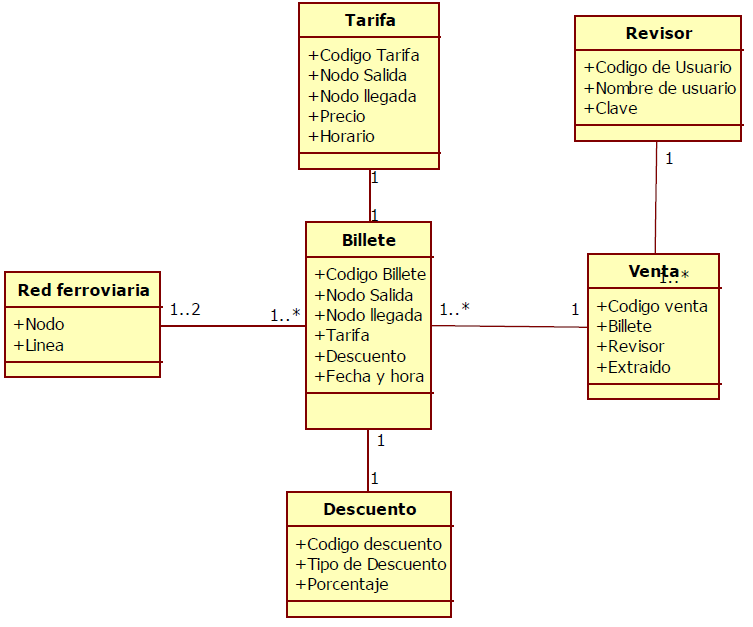
\includegraphics[width=0.7\linewidth]{./captura}
\label{fig:captura}
\end{figure}


Todos los datos serán alfanuméricos, sin embargo, el password deberá almacenarse de forma encriptada.\\

En términos de rendimiento, la base de datos debe alinearse con los requisitos de rendimiento de VIRUTA enunciados en la sección 3.3.\\

Dados los limitados recursos técnicos de los dispositivos, la base de datos deberá ser lo más ligera posible.

